% ----------------------------------------------------------
\chapter{Introdução}
\label{cap_intr}
% ----------------------------------------------------------
\section{Queimadas e Amazônia}
O Brasil é o país com a maior presença da floresta Amazônica na América, 60\% do total da floresta está dentro do território brasileiro, o que equivale a aproximadamente 5 milhoes de quilômetros quadrados ou 59\% do território nacional \cite{tamanhoIBGE}. Por consequência disto, possuimos uma enorme responsabilidade com ela, existente em diversas formas, como na defesa do território nacional ou na proteção de um enorme patrimônio da humanidade. 

Tal patrimônio vem requerendo cada vez mais atenção nos últimos tempos, de acordo com dados gerados pelo PRODES \cite{novatecnica}, entre agosto de 2021 e julho de 2022 a taxa de desmatamento da Amazônia Legal foi cerca de 11594$km^{2}$. Como podemos ver na figura \ref{fig:prodesgraph}, tal taxa vem acompanhando uma alta nos últimos 10 anos do desmatamento no bioma. O INPE \cite{INPE} estima que, desde 1988, 17\% do bioma já tenha sido desmatado. Tais dados reforçam a necessidade de métodos de monitoramento e controle que reduzam as perdas do meio ambiente.

\begin{figure}[htb]
	\centering
	\begin{minipage}{0.9\linewidth}
		\centering
		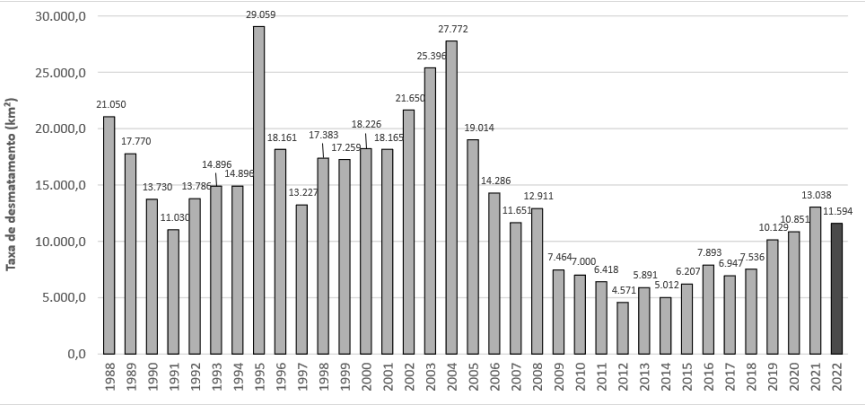
\includegraphics[width=\linewidth]{tg1/figuras/prodes.png}
		\caption{Taxas consolidadas anuais de desmatamento do PRODES \cite{novatecnica}}
            \label{fig:prodesgraph}
	\end{minipage}
\end{figure}

Uma importante área de atuação na preservação da floresta se trata do combate à incêndios. Todos os anos, milhares de quilômetros da floresta amazônicas são queimados por incêndios florestais, causando impactos ecológicos e econômicos, redução da biomassa florestal, mudanças na composição de espécies de árvores e esgotamento do solo \cite{penha}. 

Os incêndios podem ocorrer naturalmente ou podem estar atrelados à atividades humanas. No entanto, queimadas resultantes da ação humana constituem quase que a totalidade dos incêndios registrados nos territórios no Brasil, ocupando o 5º lugar entre os países mais poluidores \cite{bdqueimadas}.

Já as queimadas naturais, por sua vez, costumam ter sua ignição dada por raios, tornando-as mais comuns em períodos de secas prolongadas quando as queimadas costumam atingir seu pico. São mais frequentes no bioma Cerrado que é naturalmente mais seco e adaptado a queimadas naturais recorrentes, normalmente no início e fim das estações chuvosas. Em contraste, o bioma Amazônia é extremamente úmido e apresenta baixos índices de queimadas naturais.

Conforme pesquisas recentes \cite{amazonia_carbono}, a queima e o desflorestamento excessivo na floresta Amazônica está afetando a capacidade de absorção de CO2 da atmosfera, ao mesmo tempo que estas atividades emitem grandes quantidades de carbono por meio da queima de madeira. Além disso, estas ações apresentam um impacto climático na região, tornando a estação seca mais seca, quente e longa, agredindo ainda mais o bioma.

\section{História do Monitoramento da Amazônia por meio de Sensoreamento Remoto}

Devido ao valor da Amazônia e da necessidade em protegê-la, é natural o interesse em se desenvolver tecnologias de monitoramento visando preservar este grande patrimônio natural. A história do sensoreamento remoto na região data desde o ano 1975, quando foram-se produzidas as primeiras imagens de satélite Landsat, por meio de um sensor MSS ou sensor multi espectral.  Estas imagens compuseram o primeiro grande mapeamento do território para se verificar o potencial desta tecnologia no monitoramento de desflorestamento.

A experiência contemplou uma área de 55 milhões de hectares referentes a uma região crítica ligada a grandes projetos agropecuário, revelando que 10\% do território já estava desflorestado. Diante da indignação internacional oriunda deste conhecimento, as autoridades brasileiras instauraram uma Comissão Parlamentar de Inquérito, ou CPI, para investigar o tema \cite{hist_amz}. 

Em contrapartida, as imagens coletadas para este estudo contemplavam apenas uma parte crítica do território, levantando a dúvida sobre o estado do resto do território. Em 1988, teve origem o projeto PRODES Analógico (Projeto de Monitoramento do Desmatamento na Amazônia Legal por Satélite), produzindo métricas desmatamento anuais para todo o território amazônico até 2003.

\begin{figure}[htb]
	\centering
	\begin{minipage}{0.9\linewidth}
		\centering
		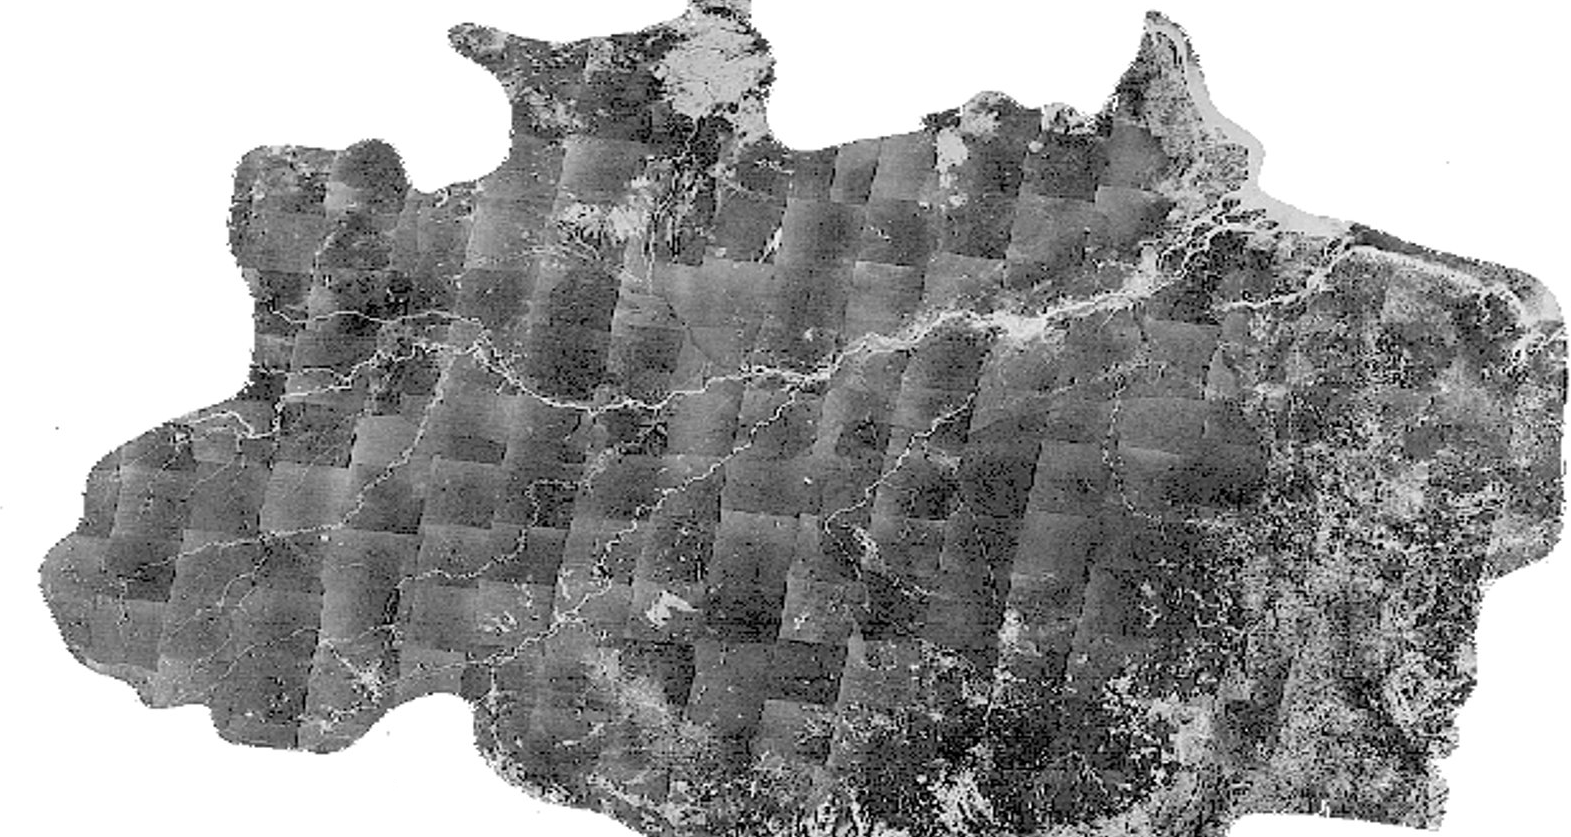
\includegraphics[width=\linewidth]{tg1/figuras/amazon.png}
		\caption{Mosaico com 229 imagens Landsat em escala 1: 250.000 \cite{hist_amz}} \label{fig:amz1988}
	\end{minipage}
\end{figure}

Em sequência, há o nascimento do projeto PANAMAZÔNIA I \cite{panamazonia} em 1992, operando de forma semelhante ao PRODES Analógico. Este novo projeto também faria o monitoramento da amazônia de forma analógica com imagens do satélite Landsat de resolução 1:250.000, visando aumentar a escala e fazer o monitoramento para toda a América do Sul. 

A próxima etapa desta história se da em 1997 por meio do PRODES Digital. Este representou um grande avanço tecnológico na forma da criação de um banco de dados digital, porém, foi limitado a operar dentro da complexidade do projeto PRODES Analógico. Por consequência disto, varias melhorias ao sistema de monitoramento e classificação não foram aplicadas.

A partir de 2003 tem-se a origem do projeto DETER (Detecção do Desmatamento em Tempo Real) \cite{deter}. Esta nova empreitada utilizou imagens do sensor MODIS, abordo do satélite Terra. Apesar da baixa resolução das imagens, tinha-se uma alta taxa de amostragem, gerando-se imagens diárias. A partir disto, o sistema fazia a sobreposição destas imagens e polígonos de desmatamento detectados. Caso um polígono de desmatamento fosse sobreposto a uma imagem de vegetação anteriormente intocada, era gerado um alerta de alteração da cobertura vegetal para os órgãos de fiscalização de desmatamento oficiais. Este foi o primeiro sistema de monitoramento em tempo quase real do território amazônico e opera até hoje.

Em 2020 foi lançado pelo Global Fire Emission Database o \textit{Amazon Dashboard}, uma ferramenta que rastreia incêndios individuais na região da Amazônia usando uma abordagem para agrupar e classificar as detecções ativas em diferentes tipo de incêndio. O GFED é um banco de dados focado em informações de incêndio obtidos por meio de satélites da NASA \cite{gfed}. No atual estado da arte, o GFED é o único dado a nível mundial com distribuição gratuita na internet que faz referência sobre tipos de fogo. 

Em 2021, o Centro Gestor e Operacional do Sistema de Proteção da Amazônia desenvolve o Painel do Fogo, uma plataforma Web que permite visualizar informações em tempo real sobre incêndios florestais na região da Amazônia com o intuito de subsidiar o acionamento de brigadas ou batalhões durante o combate ao fogo. A novidade se baseia em trabalhar agrupamentos de focos de calor para entender se tal situação é um evento individual de incêndio e queimada, e disponibilizá-los no Mapa Interativo de Incêndios e Queimadas \cite{painel-fogo}. Embora 



%No entanto, a floresta Amazônica compreende um território extremamente extenso com uma mata bastante fechada, implicando em um desafio prático e logístico em sua proteção e monitoramento.

%\todo{tem que readaptar muita coisa}



\section{Justificativa e Objetivos}

\todo{Painel do Fogo - O que é e integração de nosso trabalho}

Os incêndios florestais de origem antropológica são predominantemente e principalmente ligados ao desmatamento e a agricultura de manutenção \cite{severidade}. Nem todo fogo iniciado por atividade humana resultará em tragédia, mas a frouxidão das leis de proteção ambiental estimula pessoas mal intencionadas a queimar grandes áreas públicas para grilagem \cite{jornal_ambiental}, então ser capaz de controlar queimadas é importante tanto para proteger os bens naturais quanto para garantir a aplicação da legislação.

A velocidade e a eficiência na detecção e monitoramento dos incêndios florestais são 
fundamentais para a viabilização do controle do fogo, e para isso é necessário possuir informações confiáveis da localidade e da área da queimada \cite{batista}. Visto a importância da preservação do território amazônico, este projeto se dispõe a desenvolver um sistema capaz de classificar por meio de algoritmos de aprendizado de máquina e de dados de satélites esses incêndios. Compondo um sistema inteligente de monitoramento para todo o território Amazônico.

De acordo com \cite{naqa}, “aprendizado de máquina é um ramo em evolução de algoritmos computacionais que são projetados para emular a inteligência humana aprendendo com o ambiente circundante."  Além disso, “pode melhorar automaticamente através da experiência” \cite{coogan}. Ao escolhermos desenvolver a ferramenta por meio de algoritmos de aprendizado de máquina, temos o objetivo de que ela possa fazer de maneira autônoma um trabalho de monitoramento que até então precisava da supervisão de um ser humano. % como fora feito anteriormente por muitos anos em projetos como o PRODES Analógico.

O algoritmo desenvolvido neste trabalho foi projetado para ser incluído ao Painel do Fogo, uma plataforma Web que disponibiliza informações sobre incêndios e queimadas no Brasil, desenvolvido pelo Centro Gestor e Operacional do Sistema de Proteção da Amazônia \cite{painel-fogo}. No entanto, diferente de outras plataformas de monitoramento, o Painel do Fogo trabalha ao lado de batalhões e brigadas no combate ao fogo. Através desta plataforma se é possível obter o 'perímetro' e o “status” mais recente sobre uma queimada ou incêndio de modo que um evento esteja associado a uma ocorrência ou acionamentos de equipes.

É importante salientar que um diferencial dos dados oferecidos pelo Painel do Fogo é a capacidade de monitorar o que chamam de eventos de fogo, observando a evolução de um incêndio ao longo do tempo através de várias detecções de focos de incêndio em proximidade. Dessarte, se é possível analisar um incêndio florestal como um evento variante no tempo.

\todo{mano, mudar né? a gente não quer fiscalizar de fato mas classificar apenas né, não identificar}

%Semelhante ao projeto DETER, este projeto visa criar uma ferramenta de monitoramento automático e quase em tempo real do território amazônico, porém, para a tipificação e prevenção de queimadas. De acordo com o \textit{EU Horizon 2020 Work Programme} \cite{horizon}, o ciclo de gestão do fogo pode ser amplamente segmentado em três etapas: (1) prevenção e preparação (pré-fogo); (2) detecção e resposta (gestão de incêndios florestais ativos); (3) atividades de restauração e adaptação (pós-incêndio). Este trabalho estará focado em desenvolver uma ferramenta que sirva de auxílio para a segunda etapa, na resposta dos órgãos de defesa para com incêndios ativos.

Dessa forma, este projeto visa criar uma ferramenta de tipificação automática de incêndios no território amazônico para auxiliar no combate ao fogo na região. De acordo com o \textit{EU Horizon 2020 Work Programme} \cite{horizon}, o ciclo de gestão do fogo pode ser amplamente segmentado em três etapas: (1) prevenção e preparação (pré-fogo); (2) detecção e resposta (gestão de incêndios florestais ativos); (3) atividades de restauração e adaptação (pós-incêndio). Este trabalho estará focado em desenvolver uma ferramenta que sirva de auxílio para a segunda etapa, na resposta dos órgãos de defesa para com incêndios ativos, através de sua integração ao Painel do Fogo.

Para este fim, a plataforma fará uso de sistemas de aprendizado de máquinas para tipificar queimadas em curso, integrando estas informações à plataforma Web. Através dela, as informações são disponibilizadas para todos que tenham interesse e alertas serão emitidos para os agentes competentes conforme a necessidade.

O uso de inteligência artificial para cuidados durante o ciclo do fogo não são uma novidade, em \cite{invention} foi feita uma revisão de diversos artigos publicados entre 2019 e 2022 que tratavam do uso de métodos de aprendizado de máquina no controle de queimadas florestais. O que se pode concluir da revisão é que existe um potencial para a adoção de métodos de aprendizado de máquina para previsão e classificação e para melhorar o suporte às decisões gerais no monitoramento de danos ambientais relacionados ao fogo.

O Painel do Fogo já possui atualmente capacidade de tipificar seu banco de dados com as quatro classificações de queimadada também utilizado pelo GFED \cite{andela}, porém nenhuma das duas ferramentas conseguem entregar tais informações em tempo real. O projeto deverá ser capaz de realizar tal trabalho de forma ligeira e com um bom nível de acurácia.

O sistema foi treinado utilizando o extenso banco de dados de queimadas no território Amazônico oferecido pelo CENSIPAM. Este dataset foi construído a partir de diversas fontes como FIRMS e VIIRS, e classificado de acordo com o próprio CENSIPAM e dados do GFED \textit{Amazon Dashboard}. Estes dados são tratados e alimentados a um algoritmo de aprendizado de máquina para o treinamento. O modelo finalizado é capaz de classificar queimadas dentro das quatro classificações utilizadas pelo CENSIPAM e pelo GFED para tipificar incêndios florestais na amazônia \cite{andela}: 

%O sistema foi treinado utilizando o extenso banco de dados de queimadas no território Amazônico oferecido pelo Amazon Dashboard do GFED \cite{gfed}. Estes dados são tratados e alimentados a um algoritmo de aprendizado de máquina para o treinamento. O modelo finalizado é capaz de classificar queimadas dentro das quatro classificações utilizadas pelo GFED para tipificar incêndios florestais \cite{andela}: 

\begin{itemize}
    \item  \textbf{Savana e pastagem}: vegetação de porte baixo, com pouca presença de biomassa, longa duração dias-semanas;
    \item \textbf{Pequenas clareiras}: pequenos incêndios em sistemas florestais (cobertura de árvores > 50$\%$ e igual ou inferior a 5 detecções de incêndios), curta duração, área menor que 100 ha;
    \item \textbf{Sub-bosque}: vegetação de porte arbustivo alto, Apresenta altas taxas de biomassa. Ocorre muito em borda de áreas desmatadas com floresta. Área variável, longa duração, poucos focos de calor por detecção, mesma região geográfica do desmatamento;
    \item \textbf{Desmatamento}: os incêndios de desmatamento normalmente têm alto poder radiativo inicial do fogo, pois os detritos lenhosos empilhados levam a uma maior liberação de energia e longa persistência do fogo, uma vez que essas pilhas podem arder por dias. Maior poder radiativo no início, maior duração, área variável.

\end{itemize} 

%Nosso objetivo é gerar nossa própria abordagem de tipificação, embora identificando os mesmos tipos de fogo e usando alguma instância de inteligência artificial, no que couber. No atual estado da arte, o GFED é o único dado a nível mundial com distribuição gratuita na internet que faz referência
%sobre tipos de fogo, mas não disponibiliza queimadas classificadas em tempo real. A diferença na data dos últimos dados disponibilizados para a data real é de cerca de um mês, propomos então um método que possa ser utilizado em tempo real para permitir rápida resposta dos órgãos de proteção ambiental.

A classificação de incêndios florestais desempenha um papel crucial na gestão ambiental, pois fornece informações essenciais para o desenvolvimento de estratégias de prevenção e combate ao fogo. Ao tipificar os incêndios dentro dessas categorias, as autoridades podem avaliar a ameaça que representam para a biodiversidade, comunidades humanas e ecossistemas. Essa análise permite a alocação eficiente de recursos, o planejamento de evacuações quando necessário e a mobilização de equipes de combate a incêndios. Além disso, a classificação de incêndios fornece dados valiosos para estudos e pesquisas que visam entender as causas subjacentes dos incêndios florestais e desenvolver medidas preventivas mais eficazes para proteger as florestas e o meio ambiente.

\section{Metodologia}

O trabalho aqui apresentado melhor se enquadra em um modelo de pesquisa experimental, onde diversas técnicas de machine learning, processamento de dados, e engenharia de features foram testadas com o objetivo de comparar a eficiência entre elas e como cada elemento é capaz de influenciar no desempenho do algoritmo.

Neste estudo, dados públicos disponíveis gratuitamente na internet foram utilizados como amostras e features para o treinamento da rede. Os dados são disponibilizados por fontes confiáveis e renomadas, utilizadas mundialmente por pesquisadores e órgãos governamentais. Para treinamento foram utilizadas amostras e informações referentes ao ano de 2020, porém as fontes dos dados são capazes de liberar novos dados frequentemente de forma que o produto final sempre se mantenha atualizado com os conhecimentos mais recentes, podendo entregar suas previsões em tempo real sem que elas percam relevância com o passar do tempo.

Como mencionado anteriormente, a qualidade e significância de cada dado dentro do projeto foi analisada experimentalmente. Normalmente ao trabalhar com machine learning e redes neurais é possível medir o quanto que cada informação está sendo importante para as tomadas de decisões do modelo. Realizando tal analise foi-se capaz de definir quais informações deveríamos priorizar a obtenção, e quais não possuiam impacto, assim como quais modelos de aprendizado de máquina aprezentavam melhor desempenho.

Com os resultados preliminares, a próxima etapa é investir em um modelo promissor e criar um código funcional que seja capaz de receber um banco de dados, povoá-lo com as features necessárias e então retornar a saída de forma que ela possa ser incorporada de volta ao banco de dados com o máximo de independência.

A eficácia final do trabalho foi medida tomando como referência o padrão estabelecido pelo CENSIPAN para tipificação de incêndios. Ele também está responsável pela revisão do produto e averiguação de sua utilidade.

%\begin{mdframed}[style=defnSty] % azul
%\begin{mdframed}[style=plainSty] % verde

%{\center \textsc{Texto motivador} \par}

%\noindent Esperamos que o \abnTeX\ aprimore a qualidade do trabalho que você produzirá, de modo que o principal esforço seja concentrado no principal: na contribuição científica.
   
%\end{mdframed}